\clearpage % Rozdziały zaczynamy od nowej strony.
\section{Wstęp}
Wyznaczenie orbity obiektu kosmicznego polega na określeniu wektora stanu (położenia oraz prędkości) obserwowanego ciała na podstawie zbioru obserwacji \cite{FiftyYears}. Zagadnienie to jest jednym z najważniejszych zadań mechaniki nieba już od początków istnienia tej dziedziny nauki. Pierwsze skuteczne metody zostały opracowane na przełomie XVIII i XIX wieku m.in. przez Laplace'a \cite{Branham2005} oraz Gaussa, który wykorzystując swoją metodę wyznaczył orbitę Ceres \cite{Teets1999}.

Współcześnie znajomość orbit potrzebna jest nie tylko do katalogowania Układu Słonecznego, ale również do planowania manewrów orbitalnych, korekcji orbit satelitów, unikania kosmicznych śmieci. Mimo upływu lat, historyczne metody w rozwiniętej wersji wciąż są wykorzystywane jako pierwsze przybliżenie dla metod numerycznych pozwalających wyznaczyć dokładniejsze rozwiązania \cite{FiftyYears}.

\subsection{Definicja wektora stanu i elementów orbitalnych}
\label{ch:wektory-stanu}
\label{wektory}
Wektor stanu orbitalnego statku kosmicznego składa się z wektorów położenia ($\mathbf{r}$) i prędkości ($\mathbf{v}$). Zgodnie z konwencją ruch statków kosmicznych w okolicy Ziemi opisuję się względem układu ECI (Earth-Centered Inertial). Jego środek znajduje się w środku Ziemi, płaszczyzna XY jest zgodna z płaszczyzną równika, oś X wskazuje na Punkt Barana, a oś Z jest zgodna z osią obrotu planety. Oś Y dopełnia układ tak, by był on prawoskrętny.  

Korzystając z prawa powszechnego ciążenia oraz drugiej zasady dynamiki można wyznaczyć równania różniczkowe ruchu obiektu i je rozwiązać, używając wektora stanu jako warunku brzegowego. Prowadzi to do wyznaczenia orbity możliwej do opisania przy pomocy elementów orbitalnych, czyli zestawu sześciu wielkości, pięciu stałych w czasie opisujących jej tor oraz szóstej, zmiennej, wskazującej aktualne położenie obiektu na orbicie \cite{CurtisWektorStanuWOE}. 
% Standardowy parametr grawitacyjny to iloczyn stałej grawitacyjnej i sumy mas ciała orbitującego i centralnego. Jest on powiązany z prawem powszechnego ciążenia Newtona. 
% \begin{equation}
% F = \frac{G(Mm)}{r^2}
% \end{equation}
% \begin{equation}
% \mu = G(M+m) \stackrel{M >> m}{\approx} GM
% \end{equation}
% Dysponując wektorem stanu ciała orbitalne obiektu, czyli zestaw wielkości pozwalających na zdefiniowanie jego orbity w modelu keplerowskim \cite{CurtisWektorStanuWOE}. 
Klasyczne elementy orbitalne składają się z:
\begin{itemize}
 \item półosi wielkiej (a)
\item inklinacji (i)
\item długości węzła wstępującego ($\Omega$)
\item mimośrodu (e)
\item argumentu perygeum ($\omega$)
\item anomalii prawdziwej ($\nu$)
\end{itemize}
Elementy orbitalne oraz układ ECI ilustruje rysunek \ref{fig:elementy-szkic}.



    \begin{figure}[h]
    \centering
    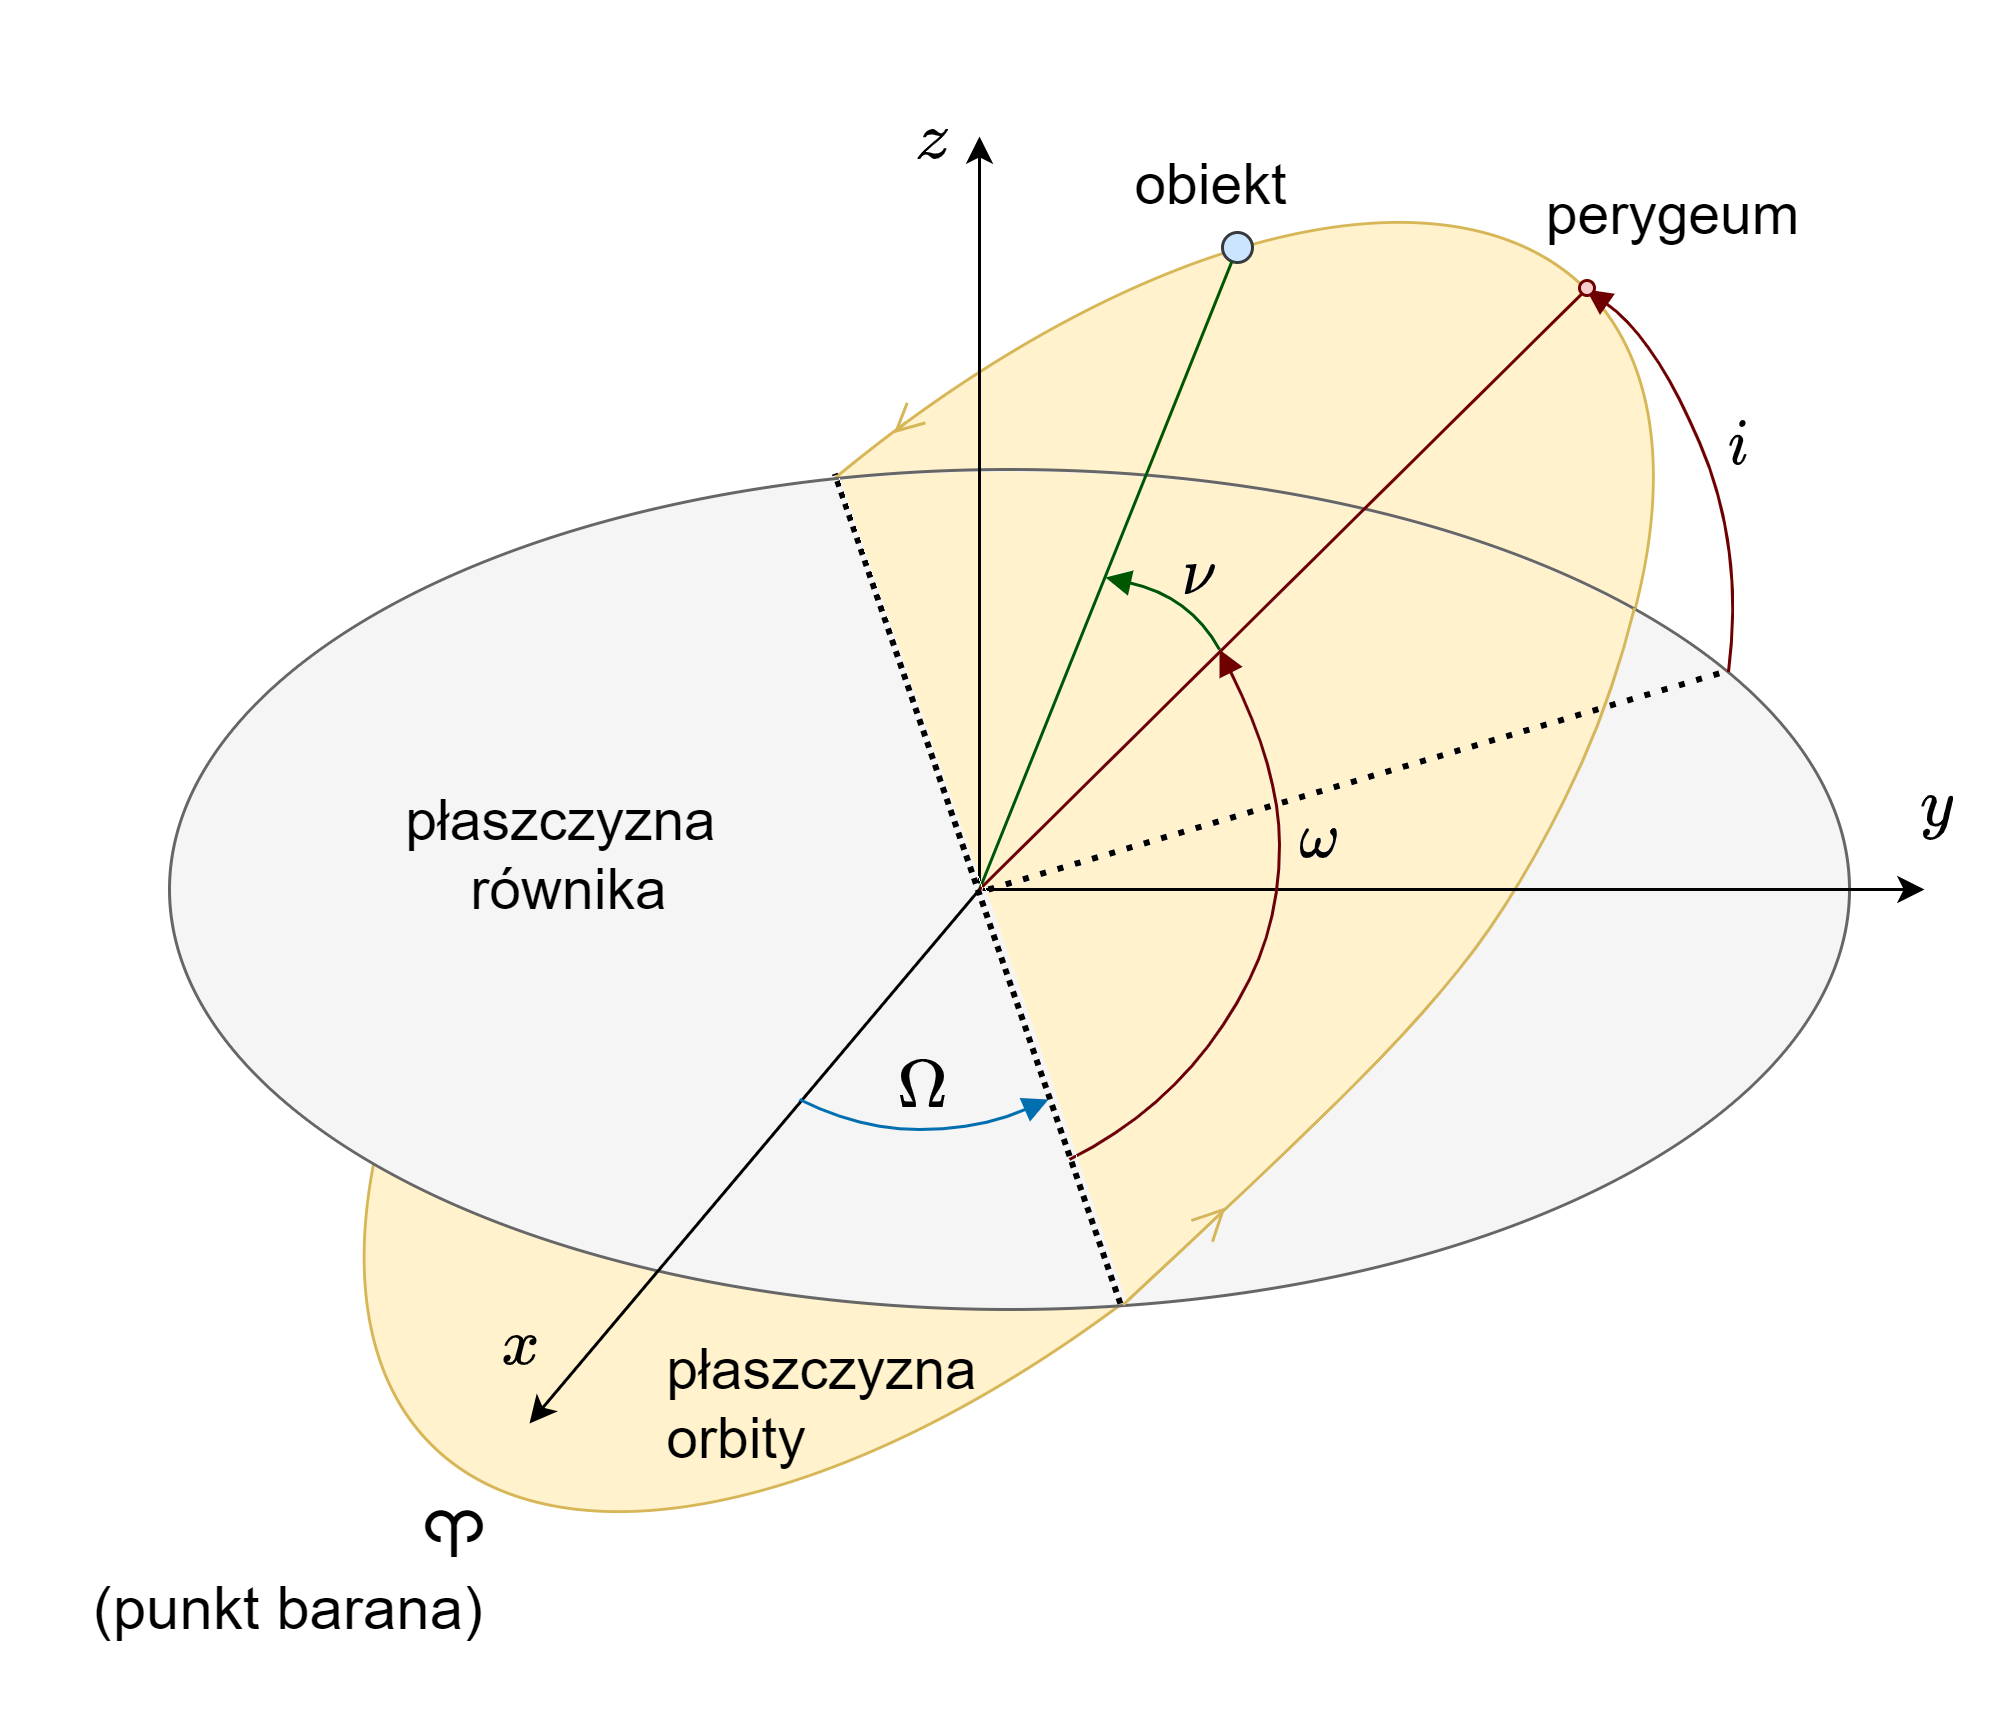
\includegraphics[width=\textwidth]{tex/img/diagramelementy.png}
    \caption{Układ referencyjny ECI oraz część elementów orbitalnych: inklinacja $i$, długość węzła wstępującego $\Omega$, argument perygeum $\omega$ i anomalia prawdziwa $\nu$}
    \label{fig:elementy-szkic}
    \end{figure}


\subsection{Transformacja wektora stanu na elementy orbitalne}
Dysponując wektorem stanu (wektor położenia $\mathbf{r}$ i wektor prędkości $\mathbf{v}$ w układzie ECI) można wyznaczyć elementy orbitalne. Potrzebny jest też powiązany z prawem powszechnego ciążenia standardowy parametr grawitacyjny $\mu$, będący iloczynem stałej grawitacyjnej i sumy mas ciała orbitującego i centralnego.
\begin{equation}
\mu = G(M+m) \stackrel{M >> m}{\approx} GM
\end{equation}

Procedura wyznaczenia elementów orbitalnych z wektora stanu: \newline
Wyznaczenie momentu pędu:
\begin{equation}
\mathbf{h} = \mathbf{r} \times \mathbf{v}
\end{equation}
 Wyznaczenie inklinacji:
\begin{equation}
i = \cos^{-1}{\left(\frac{h_z}{\|\mathbf{h}\|}\right)}
\end{equation}
 Wyznaczenie: osi apsyd i długości węzła wstępującego:
\begin{align}
\mathbf{N} &= [0,0,1] \times \mathbf{h} \\
\Omega &= \cos^{-1}{\left(\frac{N_x}{\|\mathbf{N}\|}\right)}
\end{align}
 Wyznaczenie mimośrodu:
\begin{equation}
\mathbf{e} = \frac{1}{\mu}\left(\mathbf{v}\times\mathbf{h}-\mu\frac{\mathbf{r}}{\|\mathbf{r}\|}\right) 
\end{equation}
\begin{equation}
e = \|\mathbf{e}\|
\end{equation}
 Wyznaczenie argumentu perygeum:
\begin{equation}
\omega = cos^{-1}\left(\frac{\mathbf{N}\cdot\mathbf{e}}{\|\mathbf{N}\|\|\mathbf{e}\|}\right)
\end{equation}
Jeśli $e_Z$ < 0:
\begin{equation}
\omega = 360\degree - \omega
\end{equation}
 Wyznaczenie anomalii prawdziwej:
\begin{equation}
\theta = cos^{-1}\left(\frac{\mathbf{e}\cdot\mathbf{r}}{\|\mathbf{e}\|\|\mathbf{r}\|}\right)
\end{equation}
Jeśli $\mathbf{r} \cdot \mathbf{v}  < 0$:
\begin{equation}
\theta = 360\degree - \theta
\end{equation}
 Wyznaczenie półosi wielkiej:
\begin{equation}
r_p = \frac{h^2}{\mu}\frac{1}{1+\|\mathbf{e}\| \cos(0\degree)}
\end{equation}
\begin{equation}
r_a = \frac{h^2}{\mu}\frac{1}{1+\|\mathbf{e}\| \cos(180\degree)}
\end{equation}
\begin{equation}
a = \frac{r_p + r_a}{2}
\end{equation}

\subsection{Metoda Gaussa}
Metoda Gaussa pozwala na wyznaczenie wektora stanu obiektu na podstawie trzech obserwacji \cite{Curtis2013}. Wymaga to pomiaru składającego się z się z czasu pomiaru $t_i$, wektora położenia obserwatora $R_i$ oraz wersora kierunkowego obserwacji $\hat{\rho_i}$. Wersor kierunkowy można wyznaczyć na podstawie zaobserwowanych współrzędnych astronomicznych  \cite{Astronomiczne}. Schemat obserwacji pokazuje Rysunek. \ref{fig:obserwacja}.

    \begin{figure}[h]
    \centering
    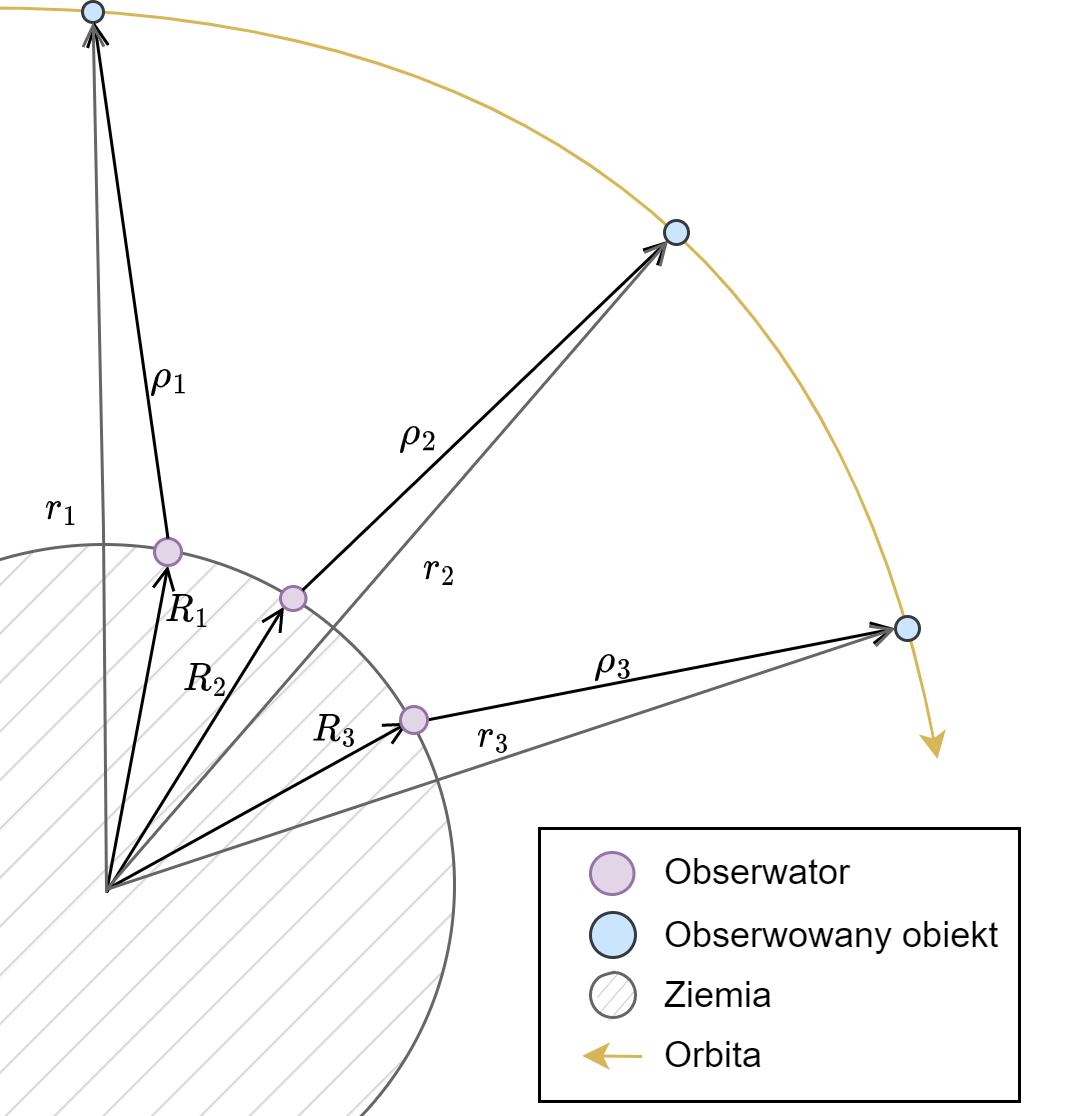
\includegraphics[width=0.8\textwidth]{tex/img/ziemia-orbita.png}
    \caption{Schemat wektorów używanych do wyznaczenia orbity metodą Gaussa}
    \label{fig:obserwacja}
    \end{figure}


Kolejne kroki metody to: \newline
Wyznaczenie międzyczasów:
\begin{align}
\tau_1 &= t_1 - t_2 \\
\tau &= t_3 - t_1 \\
\tau_3 &= t_3 - t_2 
\end{align}
Wyznaczenie iloczynów: 
\begin{align}
\mathbf{p}_1 &= \mathbf{\hat{\boldsymbol\rho}}_2 \times  \mathbf{\hat{\boldsymbol\rho}}_3 \\
\mathbf{p}_2 &= \mathbf{\hat{\boldsymbol\rho}}_1 \times  \mathbf{\hat{\boldsymbol\rho}}_3\\
\mathbf{p}_3 &= \mathbf{\hat{\boldsymbol\rho}}_1 \times  \mathbf{\hat{\boldsymbol\rho}}_2\\
D_0 &= \hat{\boldsymbol\rho}_1 \cdot \mathbf{p}_1
\end{align}
Wyznaczenie macierzy $\boldsymbol{D}_{3x3}$:
\begin{equation}
D_{ij} = \boldsymbol R_i \cdot \boldsymbol p_j
\end{equation}
Wyznaczenie współczynników A i B:
\begin{align}
A &= \frac{1}{D_0} \left(-D_{12}\frac{\tau_3}{\tau}+D_{22}+D_{32}\frac{\tau_1}{\tau}\right) \\
B &= \frac{1}{6D_0} \left(D_{12}(\tau_3^2-\tau^2)\frac{\tau_3}{\tau}+D_{32}(\tau^2-\tau^2_1)\frac{\tau_1}{\tau}\right)
\end{align}
Wyznaczenie współczynnika E: 
\begin{equation}
E = \mathbf{R}_2 \cdot \boldsymbol{\hat{\rho}}_2
\end{equation}
Wyznaczenie współczynników a, b i c:
\begin{align}
a &= -(A^2+2AE+\|\mathbf{R}_2\|^2)\\
b &= -2\mu B(A+E)\\
c &=  -\mu^2B^2 
\end{align}
Wyznaczenie rzeczywistego, nieujemnego pierwiastka wielomianu i przyjęcie go jako wartość $\|\boldsymbol{r}_2\|$:
\begin{equation}
x^8 + ax^6 + bx^3 + c = 0
\end{equation}
Wyznaczenie wartości wektora obserwacji:
\begin{align}
\|\boldsymbol\rho_2\| &= A + \frac{\mu B}{\|\mathbf{r}_2\|^3} \\
\|\boldsymbol\rho_1\| &= \frac{1}{D_0} \left(\frac{6\left(D_{31}\frac{\tau_1}{\tau_3}+D_{21}\frac{\tau}{\tau_3}\right)\|\mathbf{r}_2\|^3 + \mu D_{31} (\tau^2-\tau_1^2)\frac{\tau_1}{\tau_3}}
{6\|\mathbf{r}_2\|^3+\mu(\tau^2-\tau^2_3)}   -D_{11} \right) \\
\|\boldsymbol\rho_3\| &= \frac{1}{D_0} \left(\frac{6\left(D_{13}\frac{\tau_3}{\tau_1}+D_{23}\frac{\tau}{\tau_1}\right)\|\mathbf{r}_2\|^3 + \mu D_{13} (\tau^2-\tau_3^2)\frac{\tau_3}{\tau_1}}
{6\|\mathbf{r}_2\|^3+\mu(\tau^2-\tau^2_3)}  -D_{33}  \right) \\
\end{align}
Wyznaczenie wektora położenia:
\begin{align}
\mathbf{r}_1 &= \mathbf{R}_1 + \|\boldsymbol{\rho}_1\| \boldsymbol{\hat{\rho}}_1 \\
\mathbf{r}_2 &= \mathbf{R}_2 + \|\boldsymbol{\rho}_2\| \boldsymbol{\hat{\rho}}_2 \\
\mathbf{r}_3 &= \mathbf{R}_3 + \|\boldsymbol{\rho}_3\| \boldsymbol{\hat{\rho}}_3
\end{align}
Wyznaczenie współczynników Lagrange'a
\begin{align}
f_1 &= 1 - \frac{1}{2}\frac{\mu}{\|\mathbf{r}_2\|^3}\tau_1^2 \\
f_3 &= 1 - \frac{1}{2}\frac{\mu}{\|\mathbf{r}_2\|^3}\tau_3^2 \\
f_1 &= \tau_1 - \frac{1}{6}\frac{\mu}{\|\mathbf{r}_2\|^3}\tau_1^3 \\
g_3 &= \tau_3 - \frac{1}{6}\frac{\mu}{\|\mathbf{r}_2\|^3}\tau_3^3 \\
\end{align}
Wyznaczenie wektora prędkości:
\begin{equation}
\mathbf{v}_2 = \frac{1}{f_1g_3-f_3g_1}\left(-f_3\mathbf{r_1}+f_1\mathbf{r_3}\right)
\end{equation}

